\documentclass[hidelinks,a4paper,11pt, nofootinbib]{article}
\usepackage{geometry}
\usepackage[spanish, es-tabla]{babel}
\usepackage[utf8]{inputenc}
\usepackage[T1]{fontenc}
\usepackage{xspace}
\usepackage{xargs}
\usepackage{fancyhdr}
\usepackage{lastpage}
\usepackage{caratula}
\usepackage[bottom]{footmisc}
\usepackage{amsmath}
\usepackage{amssymb}
\usepackage{algorithm}
\usepackage[noend]{algpseudocode}
\usepackage{array}
\usepackage{xcolor,colortbl}
\usepackage{amsthm}
\usepackage{listings}
\usepackage{soul}

\usepackage{graphicx}
\usepackage{sidecap}
\usepackage{amsmath}
\usepackage{wrapfig}
\usepackage{caption}

\usepackage{endnotes}


%Formato de los links
\usepackage{hyperref}
\hypersetup{
  colorlinks   = true, %Colours links instead of ugly boxes
  urlcolor     = blue, %Colour for external hyperlinks
  linkcolor    = blue, %Colour of internal links
  citecolor   = red %Colour of citations
}

\renewcommand{\notesname}{Bibliografía}
\renewcommand{\theendnote}{\Roman{endnote}}

%%fancyhdr
\pagestyle{fancy}
\thispagestyle{fancy}
\addtolength{\headheight}{1pt}
\lhead{Aprendizaje Automático: TP1}
\rhead{$2º$ cuatrimestre de 2016}
\cfoot{\thepage\ / \pageref{LastPage}}


%%caratula
\materia{Aprendizaje Automático}
\titulo{Trabajo Práctico Número 1: Spam Filter}
%\subtitulo{}
\grupo{}
\integrante{Abdala, Leila Yasmín}{950/12}{abdalaleila@gmail.com}
\integrante{Costa, Manuel José Joaquín}{035/14}{manucos94@gmail.com}
\integrante{Bertero, Federico Alberto}{}{federico.bertero@gmail.com}

\fecha{27 de Septiembre de 2016}

\begin{document}

\maketitle


\section{Extracción de atributos}

Para esta primer etapa se planteó dos tipos de atributos, automáticos y no automáticos. Los atributos no automáticos son 4. HTML, de tipo binario que indica si un mail contiene código HTML. SUBJ, de tipo binario que indica si un mail contiene el campo subject. LEN, de tipo entero que retorna la cantidad de caracteres del mail. Y finalmente SPACES, de tipo entero cuenta la cantidad de espacios de la forma `` '' que parecen en el mail.

Los atributos automáticos básicamente son un vocabulario de palabras frecuentes.

En un primer intento se trató de extraer atributos de forma más sofisticada: por ejemplo, tener un vocabulario de palabras frecuentes en el body, otro del subject y realizar stemming para números. Una necesidad que surgía con esto era la de preprocesar los mails, entre otras cosas eliminando las etiquetas HTML, pues un alto porcentaje de los mails de Spam tenían contenido HTML y esto ocasionaba que dichas etiquetas dominaran el ranking de palabras frecuentes, generándose así un solapamiento con la información aportada por el atributo binario HTML. El problema que nos encontramos con esto fue que el HTML tenía un formato extraño que provocaba que las herramientas standard de procesamiento de HTML funcionaran mal.

Así mismo era importante poder eliminar palabras comunes que no aportan información como conectores, preposiciones y pronombres (the, he, she, why, etc.).

Otra complicación era con el preprocesamiento de los headers, pues los formatos de los distintos mails no eran totalmente homogéneos (por ejemplo, algunos tenían subject y otros no).

Debido a nuestra inexperiencia en el procesamiento de texto masivo, perdimos gran cantidad de tiempo y esfuerzo para solucionar estos problemas sin lograr hallar una solución correcta y eficiente. Finalmente decidimos encarar el problema de una forma más simple, sin realizar casi nada de preprocesamiento, aprovechando las herramientas que da SKLearn\footnote{Agregar link!!!!}.

La solución paliativa que encontramos fue armar un vocabulario que solo contuviera a las palabras que aparecían en al menos un 3\% de los mails de spam (este número es arbitrario, más que nada para evitar que palabras que aparecen ínfimamente estén en el vocabulario), y en no más del 60\% (este número también es arbitrario aunque un poco menos pues en efecto realizamos alguna experimentación manual). El truco está en que al imponer el tope del 60\% eliminamos la mayoría de código HTML, conectores y pronombres, pues los mismos tienen una frecuencia más elevada en general. En este sentido se hizo una suposición \emph{naive} sobre la frecuencia de aparición de las \emph{keywords}: las mismas no deberían aparecer en más de un 60\% de los mails de spam. El vocabulario que se uso finalmente fue de 787 palabras (exactamente todas las palabras que cumplían las condiciones impuestas). Es importante destacar que solo se consideraron palabras formadas por letras del alfabeto inglés (no números ni símbolos) y se obtuvieron de los mails completos (es decir que no se extrajeron solo del body).

Vale destacar que entre el primer intento de obtener los atributos automáticos y el segundo, este último no solo fue más eficiente en cuanto al tiempo sino también en cuanto a los resultados del Decision Tree. Pero claramente esta es una comparación injusta pues jamás logramos realizar el preprocesamiento de la forma deseada para el primer caso. Es por eso que no reportamos resultados de este primer intento, pues no los consideramos significativos.


\section{Modelos}

A continuación, se enuncian como items, los algoritmos de aprendizaje utilizados para experimentar y como subitems, los hiper parametros elegidos para cada uno de ellos.  
\begin{itemize}
    \item Decision Tree
        \begin{itemize}
            \item \textit{max\_leaf\_nodes} $=$ 100 (\textit{max\_leaf\_nodes} $\neq$ None $\rightarrow$ anula \textit{max\_depth})
            \item \textit{max\_features} $=$ None
            \item \textit{max\_leaf\_nodes} $=$ 100
            \item \textit{min\_samples\_split} $=$ 2
            \item \textit{criterion} $=$ gini
        \end{itemize}
    \item Gaussian Naive Bayes
    \item Multinomial Naive Bayes
        \begin{itemize}
            \item \textit{alpha} $=$ 0.25 
            \item \textit{fit\_prior} $=$ True 
        \end{itemize}
    \item Bernoulli Naive Bayes
        \begin{itemize}
            \item \textit{binarize} $=$ 0.0 
            \item \textit{alpha} $=$ 0.25
            \item \textit{fit\_prior} $=$ False
        \end{itemize}
    \item K Nearest Neighbors
        \begin{itemize}
            \item \textit{n\_neighbors} $=$ 1
            \item \textit{weights} $=$ uniform
            \item \textit{leaf\_size} $=$ 15
            \item \textit{algorithm} $=$ kd\_tree
        \end{itemize}
    \item Support Vector Machines
    \item Random Forest
        \begin{itemize}
            \item \textit{kernel} $=$ rbf 
            \item \textit{C} $=$ 1 
            \item \textit{gamma} $=$ 1.0
        \end{itemize}
\end{itemize}

Para todos estos algoritmos se utilizó la implementación de la librería \textbf{sklearn} mientras que, para la elección de los mejores hiper parámetros, se hizo uso de la técnica denominada \textbf{Grid Search}, definiendo las grillas con valores que se consideraron adecuados para cada caso en particular.

Como se puede ver, dos clasificadores no tienen hiper parámetros asociados. En el primer caso, Gaussian Naive Bayes, se debe a que la implementación utilizada del mismo no soporta parametros. En el caso de Support Vector Machines, no se pudo realizar la experimentación completa debido a una mala implementación inicial y la gran tiempo que esta requiere.


\section{Reducción de dimensionalidad}
Para esta etapa, y con el fin de reducir la cantidad de atributos y mejorar la performance de los modelos, se optó por utilizar las técnicas \textbf{Select K Best} y \textbf{Principal Component Analysis}.

\textbf{Select K Best} es un método univariable para la selección de atributos. Es decir, es un método que luego de elegir una métrica de evaluación, aplica esta sobre cada atributo de forma individual, genera un rating y se queda con los $k$ mejores. Se utilizó la implementación del algoritmo de \textit{sklearn}\footnote{\url{http://scikit-learn.org/stable/modules/generated/sklearn.feature_selection.SelectKBest.html}} y como parámetros de la misma, se opto por iterar sobre la cantidad de atributos a seleccionar, $k$, y tomar como metrica de evaluación la función $chi2$\footnote{\url{http://scikit-learn.org/stable/modules/generated/sklearn.feature_selection.chi2.html}} ya que soporta una matriz sparse como entrada.

Con \textbf{Principal Component Analysis} se buscó proyectar los datos de entrada en un espacio de dimensión menor, maximizando la varianza de los datos proyectados. Para esta técnica, al igual que para la anterior, se hizo uso de su respectiva implementación en la librería \textit{sklearn}\footnote{\url{http://scikit-learn.org/stable/modules/generated/sklearn.decomposition.PCA.html}}. El parámetro de mayor importancia en este caso es $n_components$, es decir, el numero de componentes a mantener y para su elección, se hizo uso e implemento el \textit{criterio de Kaiser}, el cual se describe a continuación. El \textit{criterio de Kaiser} consiste en retener solo las componentes principales (nuevos atributos formados como combinación lineal de los atributos originales) con autovalor mayor a 1.


\section{Resultados}

Para la evaluación de los métodos, se utiliza como métrica la media armónica con $\beta = 0,5$, $f_{0,5}$, ya se desea enfatizar la precisión. Esto es porque, al estar clasificando Spam, se considera un grave error que un mail que no entra en dicha categoría sea clasificado como tal, mientras que clasificar un Spam como Ham es aceptable. Es decir, se busca penalizar con mayor rigurosidad los casos de falsos positivos sobre los casos de verdaderos negativos.

Al comenzar, se dividió el conjunto de datos de entrada en dos conjuntos: uno para entrenamiento (training set), con el 80\% de los datos de entrada, y uno para evaluación (test set), con el 20\% de los datos de entrada. En la tabla \ref{tab1} que se encuentra a continuación se puede ver el valor que se obtiene como score para cada uno de los clasificadores con los hiper parametros enunciados en la sección 2 y sin aplicar reducción de atributos, al ser entrenados sobre el training set y prediciendo sobre el test set.

\begin{table}[ht!]
\centering
    \begin{tabular}{| l | l|}
        \hline
        \multicolumn{2}{|c|}{Scores over test set} \\
        \hline
        Algoritmo & $f_{0,5}$ \\
        \hline
        Decision Tree & 0.998397578563 \\
        Gaussian Naive Bayes & 0.563328795442 \\
        Multinomial Naive Bayes & 0.646444592629 \\
        Bernulli  & 0.990909507236 \\
        KNN & 0.94193989071 \\
        \color{red}{Random Forest} & \color{red}{0.999622322936} \\
        \hline
    \end{tabular}
    \caption{Valor de la función score aplicada sobre los diferentes clasificadores}
    \label{tab1}
\end{table}

\newpage

En la figura \ref{fig1}, se puede ver como varia el accuracy obtenido al aplicar diferentes clasificadores sobre datos con diferentes $k$ atributos, seleccionados por el algoritmo Select K Best.

\begin{figure}[ht!]
    \centering
    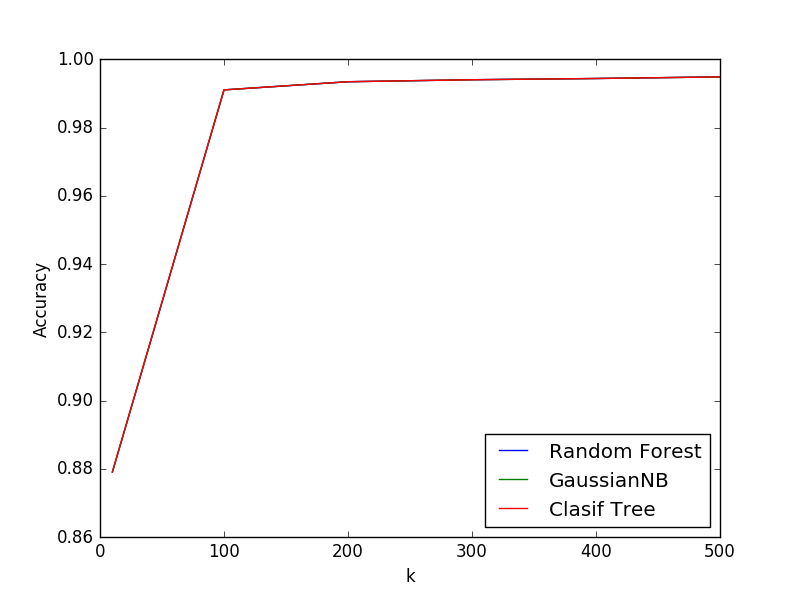
\includegraphics[width=0.8\textwidth]{k_best.png}
    \caption{Variación del accuracy en relación a la selección de $k$ atributos.}
    \label{fig1}
\end{figure}

Al aplicar el criterio de Kaiser, se obtuvo que el mejor número de componentes para utilizar como parámetro del algoritmo PCA es 142.

En la figura \ref{fig2}, se puede comparar como varia el score $f_{0,5}$ al aplicar las dos técnicas de reducción de dimensionalidad con los parámetros que resultaron mejores y sobre cada uno de los clasificadores.

\begin{figure}[ht!]
    \centering
    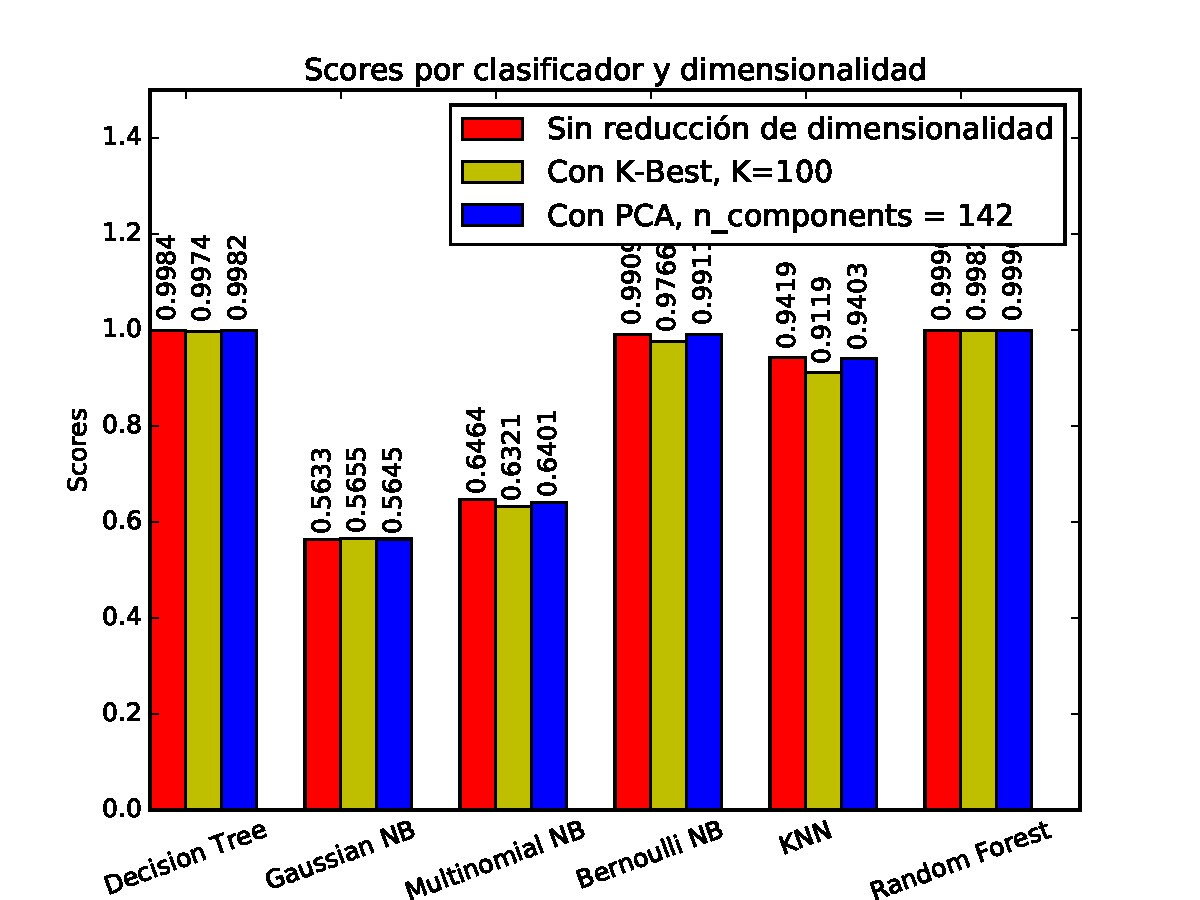
\includegraphics[width=0.8\textwidth]{barplot.pdf}
    \caption{Variación de $f_{0,5}$ en los diferentes clasificadores al aplicar las técnicas de reducción de dimensionalidad.}
    \label{fig2}
\end{figure}

\end{document}

